\mode*

\section[Book and author]{The book and author}

\begin{frame}
  \begin{figure}
    
\includegraphics[height=0.8\textheight]{fig/book.jpg}
    \caption{Front cover of Necessary Conditions of Learning.}
  \end{figure}
\end{frame}

\begin{frame}
  \begin{figure}
    
\includegraphics[width=\columnwidth]{fig/necessary-conditions-citations.png}
    \caption{Citations for the book.}
  \end{figure}
\end{frame}

\begin{frame}
  \begin{figure}
    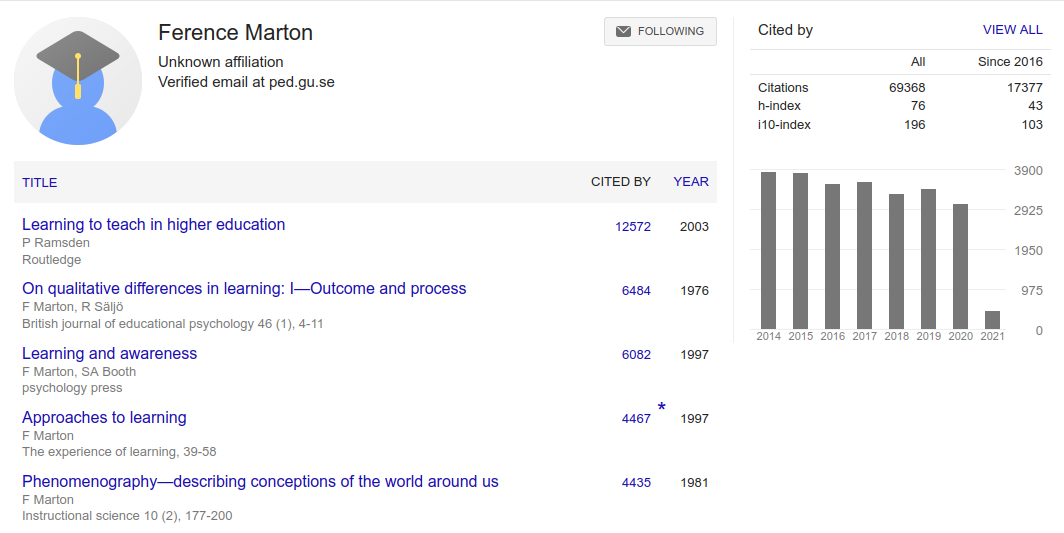
\includegraphics[width=\columnwidth]{fig/marton-gscholar.png}
    \caption{Marton's profile on Google Scholar, showing his high citation 
    counts.}
  \end{figure}
\end{frame}

\begin{frame}
  \begin{block}{Main ideas}
    \begin{itemize}
      \item Phenomenography~\cite{Phenomenography}
      \item Variation theory~\cite{VariationTheory}
      \item Learning studies~\cite{LearningStudy}
    \end{itemize}
  \end{block}
\end{frame}

\section{Phenomenography}

\begin{frame}
  \blockcquote{NecessaryConditionsOfLearning}{%
    We tacitly assume that what we see is exactly what is there to be seen and 
    that others see things in the same way we do. It is hard to realize that we 
    have actually learned to see the world in certain ways and that others may 
    have learned to see it differently.
  }
\end{frame}

\begin{frame}
  \begin{block}<1-2>{Phenomenography~\cite{Phenomenography}}
    \begin{itemize}
      \item Reality is experienced.
      \item People interpret significant aspects of reality.
    \end{itemize}
    \pause
    \begin{description}
      \item[First-order perspective] describes various aspects of the world.
      \item[Second-order perspective] describes people's experiences of various 
        aspects of the world --- phenomenography.
    \end{description}
  \end{block}
\end{frame}

\section{Variation theory}

\begin{frame}
  \begin{block}{Variation theory~\cite{VariationTheory}}
    \vspace{-0.5em}
    \[
      \text{learning}
      \quad\leftarrow\quad
      \text{discernment}
      \quad\leftarrow\quad
      \text{variation}
    \]
  \end{block}

  \pause

  \begin{remark}
    \begin{itemize}
      \item There must be a pattern of variation to experience.
      \item \emph{This pattern must be experienced}.
    \end{itemize}
  \end{remark}
\end{frame}

\begin{frame}
  \begin{block}{Patterns of variation}
    \vspace{-0.5em}
    \[
      \text{contrast}
      \quad\rightarrow\quad
      \text{generalization}
      \quad\rightarrow\quad
      \text{fusion}
    \]
  \end{block}

  \begin{figure}
    \begin{subfigure}{0.3\columnwidth}
      \centering
      \includegraphics{fig/contrast-color.tikz}
      \caption{Contrast}
    \end{subfigure}
    \hfill
    \begin{subfigure}{0.3\columnwidth}
      \centering
      \includegraphics{fig/generalization-color.tikz}
      \caption{Generalization}
    \end{subfigure}
    \hfill
    \begin{subfigure}{0.3\columnwidth}
      \centering
      \includegraphics{fig/fusion-color.tikz}
      \caption{Fusion}
    \end{subfigure}
    \caption{%
      Illustrating the patterns of variation for aspects color and shape.
    }
  \end{figure}
\end{frame}

\begin{frame}
  \begin{figure}
    \semitransp{%
      \begin{subfigure}{0.3\columnwidth}
        \centering
        \includegraphics{fig/contrast-color.tikz}
        \caption{Contrast}
      \end{subfigure}
    }
    \hfill
    \begin{subfigure}{0.3\columnwidth}
      \centering
      \includegraphics{fig/generalization-color.tikz}
      \caption{Generalization}
    \end{subfigure}
    \hfill
    \semitransp{%
      \begin{subfigure}{0.3\columnwidth}
        \centering
        \includegraphics{fig/fusion-color.tikz}
        \caption{Fusion}
      \end{subfigure}
      \caption{%
        Illustrating the patterns of variation for aspects color and shape.
      }
    }
  \end{figure}

  \begin{remark}
    \begin{itemize}
      \item We tend to focus on induction (\ie generalization without 
        contrast).
      \item \enquote{Good theses from previous years.}
      \item \enquote{One example of linear function, another example of linear 
        function.}
    \end{itemize}
  \end{remark}
\end{frame}

\section{Learning study}

\begin{frame}
  \begin{block}{Learning study~\cite{LearningStudy}}
    \begin{itemize}
      \item Design-Based Research + Variation Theory
      \item Extends the Japanese concept Lesson Study.
    \end{itemize}
    \pause
    \begin{enumerate}
      \item \label{design} (Re-)Design teaching material/plan using variation 
        theory.
      \item Perform teaching.
      \item Analyze teaching performance and student outcomes.
      \item Go to \ref{design}.
    \end{enumerate}
  \end{block}

  \pause

  \begin{remark}
    \begin{itemize}
      \item Teacher teams, teach the same thing to different classes.
      \item Yields iterations.
    \end{itemize}
  \end{remark}
\end{frame}

\begin{frame}
  \begin{example}
    \begin{itemize}
      \item I'll work systematically according to this with my TAs.
      \item Review the main material and labs (weekly modules).
      \item Two TAs, two non-parallel tutorial groups.
    \end{itemize}
  \end{example}
\end{frame}

\section{Disposition}

\begin{frame}
  \begin{enumerate}
    \item \textbf<2>{What makes humans human?}
      \hfill
      \onslide<2>{(forms of learning)}
    \item \textbf<3>{What is to be learned?}
      \hfill
      \onslide<3>{(learning objectives)}
    \item \textbf<4>{Sameness and difference in learning}
      \hfill
      \onslide<4>{(variation theory)}
    \item \textbf<5>{What does the world look like to others?}
      \hfill
      \onslide<5>{(phenomenography)}
      \setcounter{chnum}{\value{enumi}}
  \end{enumerate}
  \begin{enumerate}
    \setcounter{enumi}{\value{chnum}}
    \item \textbf<6>{The art of learning}
      \hfill
      \onslide<6>{(learning alone, doing research)}
    \item \textbf<7>{Making learning possible}
      \hfill
      \onslide<7>{(teaching)}
    \item \textbf<8>{Learning to help others to learn}
      \hfill
      \onslide<8>{(education research)}
  \end{enumerate}
\end{frame}

\subsection{Foundations}

\begin{frame}
  \begin{enumerate}
    \alert{
    \item What makes humans human?
      \hfill
      (forms of learning)
    }
    \item What is to be learned?
      \hfill
      (learning objectives)
    \item Sameness and difference in learning
      \hfill
      (variation theory)
    \item What does the world look like to others?
      \hfill
      (phenomenography)
    \item The art of learning
      \hfill
      (learning alone, doing research)
    \item Making learning possible
      \hfill
      (teaching)
    \item Learning to help others to learn
      \hfill
      (education research)
  \end{enumerate}
\end{frame}

\begin{frame}
  \begin{block}{Ch 1 What makes humans human?}
    \begin{itemize}
      \item What is pedagogy?
      \item How does it relate to learning?
    \end{itemize}
  \end{block}

  \begin{example}<2>[Learning as a by-product or as an aim]
    \begin{itemize}
      \item Apprenticeship (PhD studies?) is learning as a by-product.
      \item Schooling is learning as an aim.
    \end{itemize}
  \end{example}

  \begin{example}<3>[\enquote{De-pedagogized} learning]
    \begin{itemize}
      \item Authentic vs unauthentic learning
      \item \enquote{Real life} vs school
    \end{itemize}
  \end{example}
\end{frame}

\begin{frame}
  \begin{example}[The teacher's paradox]
    \blockcquote[p.~13]{NecessaryConditionsOfLearning}{%
      \textins{T}he more clearly the teacher tells the students what is to be 
      done, the less chance the students get to make the necessary distinctions 
      (for instance, between what is critical and what is not).%
    }
  \end{example}
\end{frame}

\begin{frame}
  \begin{center}
    What is to be learned?\\[1em]
    instead of\\[1em]
    What is to be done?
  \end{center}
\end{frame}

\begin{frame}
  \begin{enumerate}
    \item What makes humans human?
      \hfill
      (forms of learning)
    \alert{
    \item What is to be learned?
      \hfill
      (learning objectives)
    }
    \item Sameness and difference in learning
      \hfill
      (variation theory)
    \item What does the world look like to others?
      \hfill
      (phenomenography)
    \item The art of learning
      \hfill
      (learning alone, doing research)
    \item Making learning possible
      \hfill
      (teaching)
    \item Learning to help others to learn
      \hfill
      (education research)
  \end{enumerate}
\end{frame}

\begin{frame}
  \begin{block}{Ch 2 What is to be learned?}
    \begin{itemize}
      \item What is an intended learning outcome?
      \item What should it be?
      \item It depends on the learner: \emph{critical aspects, critical 
        features} --- the atoms of the learning objective.
    \end{itemize}
  \end{block}

  \pause

  \begin{block}{The goal}
    \begin{itemize}
      \item \textcquote{NecessaryConditionsOfLearning}{The focus of the theory 
        elaborated in this book is on learning to handle new situations in 
      powerful ways.}
    \end{itemize}
  \end{block}
\end{frame}

\begin{frame}
  \begin{figure}
    \begin{subfigure}{0.3\columnwidth}
      \centering
      \includegraphics{fig/contrast-color.tikz}
      \caption{Contrast}
    \end{subfigure}
    \hfill
    \begin{subfigure}{0.3\columnwidth}
      \centering
      \includegraphics{fig/generalization-color.tikz}
      \caption{Generalization}
    \end{subfigure}
    \hfill
    \begin{subfigure}{0.3\columnwidth}
      \centering
      \includegraphics{fig/fusion-color.tikz}
      \caption{Fusion}
    \end{subfigure}
    \caption{%
      Illustrating the patterns of variation for aspects color and shape.
    }
  \end{figure}

  \begin{onlyenv}<1>
    \begin{example}
      \begin{itemize}
        \item Critical aspect: colour.
        \item Critical feature: blue.
        \item Non-critical feature: green.
        \item Non-critical aspect: shape.
        \item Non-critical features: circle, square.
      \end{itemize}
    \end{example}
  \end{onlyenv}
  \begin{onlyenv}<2>
    \begin{remark}
      \begin{itemize}
        \item There are other aspects too, \emph{unintentionally}.
        \item Another aspect in this figure is order: the circle is always 
          \enquote{first} (to the right).
      \end{itemize}
    \end{remark}
  \end{onlyenv}
\end{frame}

\begin{frame}
  \begin{figure}
    \includegraphics[height=0.5\textheight]{fig/maja-writing.jpg}
    \caption{Child's writing.
      (Corresponds to~\cite[Fig.~2.1, p.~30]{NecessaryConditionsOfLearning}.)
    }
  \end{figure}
  \begin{example}
    \begin{itemize}
      \item Obviously knows some aspect(s) of writing, just not all.
      \item Even the camera app detected this as text.
    \end{itemize}
  \end{example}
\end{frame}

\begin{frame}
  \begin{enumerate}
    \item What makes humans human?
      \hfill
      (forms of learning)
    \item What is to be learned?
      \hfill
      (learning objectives)
    \alert{
    \item Sameness and difference in learning
      \hfill
      (variation theory)
    }
    \item What does the world look like to others?
      \hfill
      (phenomenography)
    \item The art of learning
      \hfill
      (learning alone, doing research)
    \item Making learning possible
      \hfill
      (teaching)
    \item Learning to help others to learn
      \hfill
      (education research)
  \end{enumerate}
\end{frame}

\begin{frame}
  \begin{block}{Ch 3 Sameness and difference in learning}
    \begin{itemize}
      \item The problem with direct reference (induction).
      \item The patterns: contrast, generalization, fusion.
      \item \textcquote[p.~71]{NecessaryConditionsOfLearning}{%
          \textins{P}racticing something other than what was tested was more 
          effective than practicing exactly what was tested.%
        }
    \end{itemize}
  \end{block}

  \begin{example}<2>[Using the known to prepare for unknown]
    \begin{itemize}
      \item Kids were to hit a target by throwing a shuttlecock (badminton 
        \enquote{ball}).
    \end{itemize}
    \begin{enumerate}
      \item Practicing from the same position as testing.
      \item Practicing from several positions, \emph{except the testing 
        position}.
    \end{enumerate}
  \end{example}
\end{frame}

\begin{frame}
  \begin{example}[Physics]
    \begin{enumerate}
      \item Students were introduced to modern physics.
      \item Students were introduced to modern physics, contrasted with what we 
        believed before.
    \end{enumerate}
  \end{example}

  \pause

  \begin{remark}
    \begin{itemize}
      \item Makes one think about history of maths.
      \item Common to have as a separate course.
      \item CS history?
    \end{itemize}
  \end{remark}
\end{frame}

\begin{frame}
  \begin{enumerate}
    \item What makes humans human?
      \hfill
      (forms of learning)
    \item What is to be learned?
      \hfill
      (learning objectives)
    \item Sameness and difference in learning
      \hfill
      (variation theory)
    \alert{
    \item What does the world look like to others?
      \hfill
      (phenomenography)
    }
    \item The art of learning
      \hfill
      (learning alone, doing research)
    \item Making learning possible
      \hfill
      (teaching)
    \item Learning to help others to learn
      \hfill
      (education research)
  \end{enumerate}
\end{frame}

\begin{frame}
  \begin{block}{Ch 4 What does the world look like to others?}
    \begin{itemize}
      \item This chapter is about phenomenography.
      \item It answers the question \enquote{how can we find out what things 
        look like to other people?}
      \item Also tells us something about assessment\footnote{%
          Marton contrasts Bloom and SOLO taxonomies and phenomenography.
        } and how to find those critical aspects.
    \end{itemize}
  \end{block}

  \pause

  \begin{example}
    \begin{itemize}
      \item \textcquote[pp.~112--113]{NecessaryConditionsOfLearning}{%
          \textins{U}nderstanding does not cause acts; instead, acts express 
          understanding.%
        }
    \end{itemize}
  \end{example}
\end{frame}

\begin{frame}
  \begin{remark}
    \begin{itemize}
      \item No one sees the world \enquote{as it is}.
      \item The world is viewed from one's own \emph{perspective}, always 
        through the lens of the self.
      \item \emph{The learner should learn to view things in more powerful 
        ways.}
    \end{itemize}
  \end{remark}

  \pause

  \begin{remark}
    \begin{itemize}
      \item Another \emph{view} of this is \enquote{mental models}.
    \end{itemize}
  \end{remark}
\end{frame}

\subsection{Theory in vivo}

\begin{frame}
  \begin{enumerate}
    \item What makes humans human?
      \hfill
      (forms of learning)
    \item What is to be learned?
      \hfill
      (learning objectives)
    \item Sameness and difference in learning
      \hfill
      (variation theory)
    \item What does the world look like to others?
      \hfill
      (phenomenography)
    \alert{
    \item The art of learning
      \hfill
      (learning alone, doing research)
    }
    \item Making learning possible
      \hfill
      (teaching)
    \item Learning to help others to learn
      \hfill
      (education research)
  \end{enumerate}
\end{frame}

\begin{frame}
  \begin{block}{Ch 5 The art of learning}
    \begin{itemize}
      \item How do people do to learn new things?
      \item Deep and surface learning
      \item Scientific discoveries as learning
    \end{itemize}
  \end{block}
\end{frame}

\begin{frame}
  \begin{enumerate}
    \item What makes humans human?
      \hfill
      (forms of learning)
    \item What is to be learned?
      \hfill
      (learning objectives)
    \item Sameness and difference in learning
      \hfill
      (variation theory)
    \item What does the world look like to others?
      \hfill
      (phenomenography)
    \item The art of learning
      \hfill
      (learning alone, doing research)
    \alert{
    \item Making learning possible
      \hfill
      (teaching)
    }
    \item Learning to help others to learn
      \hfill
      (education research)
  \end{enumerate}
\end{frame}

\begin{frame}
  \begin{block}{Ch 6 Making learning possible}
  \end{block}
\end{frame}

\begin{frame}
  \begin{enumerate}
    \item What makes humans human?
      \hfill
      (forms of learning)
    \item What is to be learned?
      \hfill
      (learning objectives)
    \item Sameness and difference in learning
      \hfill
      (variation theory)
    \item What does the world look like to others?
      \hfill
      (phenomenography)
    \item The art of learning
      \hfill
      (learning alone, doing research)
    \item Making learning possible
      \hfill
      (teaching)
    \alert{
    \item Learning to help others to learn
      \hfill
      (education research)
    }
  \end{enumerate}
\end{frame}

\begin{frame}
  \begin{block}{Ch 7 Learning to help others to learn}
  \end{block}
\end{frame}

\section{Summary}

\begin{frame}
  \begin{block}{Take aways for practice}
    \begin{itemize}
      \item Variation theory
      \item Phenomenography
      \item Learning studies
    \end{itemize}
  \end{block}

  \begin{block}{Beautiful foundation}
    \begin{itemize}
      \item Explains other learning theories, \eg Vygotsky~\cite{Vygotsky}.
      \item Takes other papers' results, explain them with the theory.
    \end{itemize}
  \end{block}
\end{frame}

\begin{frame}
  \begin{alertblock}{Conjecture}
    \begin{itemize}
      \item OLI works due to the quiz-question feedback yields \emph{contrast}.
      \item Material usually focus on induction (\emph{generalization} without 
        contrast).
      \item \Ie students get the necessary pattern of variation.
    \end{itemize}
  \end{alertblock}
\end{frame}

\begin{frame}
  \begin{alertblock}{Conjecture}
    \begin{itemize}
      \item Students need to repeat things 8 times to learn.
      \item That's how many times they need to discern the critical 
        aspects/features.
      \item With properly designed material\footnote{%
          With the possibility to experience the necessary patterns of 
          variations.
        }, this number can be reduced.
    \end{itemize}
  \end{alertblock}
\end{frame}

\begin{frame}
  \begin{block}{Ending quote}
    \textcquote[p.~246, my emphasis]{NecessaryConditionsOfLearning}{%
          \enquote{Top scores from Shanghai stun educators,} wrote the 
          \emph{New York Times} on December 7, 2010.
          \textelp{}
          A number of different explanations were presented in the article 
          \textins{by journalists, politicians, education experts}.
          Interestingly, there was not a single word said about the things that 
          this whole book is dealing with: how the different subjects are 
          learned and taught. \emph{Could it not be the case that students are 
            better at solving quadratic equations because they are taught to 
          solve quadratic equations in more powerful ways?}%
        }
  \end{block}
\end{frame}

